\documentclass{article}
\usepackage{spconf,amsmath,amssymb,graphicx,booktabs,bm}
\usepackage[hidelinks]{hyperref}

% ---- result macros (set from results/*.json; see scripts/paper_numbers.py) ----
\newcommand{\dipQRS}{0.92}      % NORM QRS dipolar fraction
\newcommand{\dipST}{0.74}       % NORM ST  dipolar fraction
\newcommand{\dipP}{0.58}        % NORM P   dipolar fraction
\newcommand{\kapSpan}{3.1}      % kappa {I,II,V2}
\newcommand{\kapColl}{4.9}      % kappa {V1,V2,V3}
\newcommand{\kapCopl}{3.9\!\times\!10^{5}}  % kappa {I,II,III}
\newcommand{\kapLimb}{6.7\!\times\!10^{4}}  % kappa limb-6
\newcommand{\genCorr}{0.00}     % generative non-dipolar correlation
\newcommand{\olsCorr}{0.28}     % OLS non-dipolar correlation (median)
\newcommand{\covEmp}{0.90}      % Mondrian-CQR empirical coverage
\newcommand{\ffRate}{0.10}      % false-flag rate

\title{Certified Reduced-Lead ECG Reconstruction:\\
What Is Recoverable, and What Is Fabricated}

\name{Anonymous}
\address{Anonymous}

\begin{document}
\maketitle

\begin{abstract}
Reconstructing missing electrocardiogram (ECG) leads from a reduced set is an
ill-posed inverse problem. The literature reports a point reconstruction and an
aggregate error; generative reconstructors, tuned for realism, can \emph{fabricate}
clinically decisive morphology---a phantom ST elevation, an invented fractionated
QRS---while the global error looks fine. We give a per-feature, per-lead
\emph{recoverability certificate}. Its core is a physical fact that generic
inverse-problem theory lacks: the ECG is, per waveform segment, an approximately
rank-3 cardiac \emph{dipole} plus a non-dipolar residual. This yields (i) a
closed-form \emph{positive} guarantee---the dipolar projection of every lead is
exactly recoverable when the observed leads span the dipole, with a per-configuration
noise gain $\kappa_s(S)$; (ii) a distribution-free \emph{calibrated} interval for the
population-predictable non-dipolar part; and (iii) a \emph{guaranteed} flag for the
observation-independent part, whose false-flag rate is controlled at level $\alpha$.
On PTB-XL, reconstructors with near-identical RMSE are shown to differ sharply under
the certificate: a generative model places large energy in the certified-unrecoverable
subspace that is \emph{uncorrelated with truth} (correlation $\approx\genCorr$), whereas
a linear baseline recovers genuine non-dipolar content. The certificate catches
fabricated ST elevations that would drive false STEMI calls, and its guarantees are
distribution-free where the physics is and only degrade, measurably, where it is not.
\end{abstract}

\begin{keywords}
electrocardiography, inverse problems, identifiability, conformal prediction,
trustworthy machine learning
\end{keywords}

\section{Introduction}
\label{sec:intro}

Wearable and reduced-lead ECG acquisition makes lead \emph{reconstruction}
ubiquitous: recover the standard 12 leads from one, three, or six observed leads.
Dozens of recent methods---linear, U-Net, transformer, and diffusion---report low
mean-squared error \cite{gradowski2025reveals,cardoso2024bayesian}. Yet a low
aggregate error certifies nothing about \emph{which} morphological features are
trustworthy. Generative reconstructors optimise realism, and by the
perception-distortion tradeoff \cite{blau2018perception} realism on an ill-posed
inverse problem is bought by \emph{inventing} content. On an ECG this is not a
cosmetic artifact: a fabricated ST-segment deviation is a fabricated diagnosis.

A recent line of work formalises hallucination in generic inverse problems
$\bm y=\bm A\bm x+\bm n$ and gives distribution-free assessment
\cite{gottschling2026hallucinations,kim2025distshift}. Porting that machinery to
ECG would be incremental: its lower bounds hold for \emph{arbitrary} $\bm A$ and say
only that ``something is unrecoverable.'' The ECG is special. Its forward operator
carries a \emph{physical} structure---a low-rank dipole and a physically meaningful
non-dipolar null space---absent from a generic $\bm A$. This lets us make a
\emph{positive}, closed-form statement (which named cardiac feature, on which lead,
is recoverable and with what noise gain) that the generic theory cannot, and to
\emph{name} the unrecoverable content physically and meter it clinically.

\noindent\textbf{Contributions.} (1) A per-segment operator decomposition of
reduced-lead ECG into three tiers---provably recoverable (dipolar), statistically
recoverable, and provably unrecoverable---with a closed-form per-configuration noise
gain $\kappa_s(S)$ that explains why $6$ coplanar limb leads recover the dipole far
worse than $3$ well-chosen leads (Sec.~\ref{sec:cert}). (2) A certified estimator:
group-conditional conformalised quantile regression for the recoverable non-dipolar
part, and a conformal-risk-controlled hallucination flag for the unrecoverable part
(Sec.~\ref{sec:calib}). (3) Evidence on PTB-XL that RMSE-matched reconstructors are
separated by the certificate---the generative model fabricates non-dipolar content
uncorrelated with truth---and that flagging prevents false STEMI calls, with
distribution-free guarantees quantified across device shift (Sec.~\ref{sec:exp}).

\section{The Recoverability Certificate}
\label{sec:cert}

\textbf{Lead algebra.} The standard 12-lead vector $\bm L\in\mathbb{R}^{12}$ has
algebraic rank $8$: the six limb leads are fixed linear combinations of $\{$I, II$\}$
(Einthoven, Goldberger), so $\bm L=\bm T\bm x$ with a known $\bm T\in\mathbb{R}^{12\times8}$
and $\bm x=[$I, II, V1--V6$]$. Observing a lead subset $S$ is exact row selection
$\bm y_S=\bm{\mathrm{Sel}}_S\bm L$; the operator is \emph{known}, so we never estimate it.

\textbf{Dipolar coordinates.} Within a waveform segment $s\in\{$P, QRS, ST, T$\}$ the
instantaneous potential is approximately a rank-3 cardiac dipole. We estimate a
per-segment dipolar basis $\bm M_s\in\mathbb{R}^{12\times3}$ (top-3 left singular
vectors of the population, segment-$s$ lead covariance) and mean $\bm\mu_s$, and write
$\bm L_s=\bm\mu_s+\bm M_s\bm d+\bm r_s$ with $\bm r_s$ the non-dipolar residual. We do
\emph{not} assume exact rank 3; $\bm M_s$ is a coordinate system and the residual is
handled by calibration. On PTB-XL the dipolar fraction is
$\dipQRS$ for QRS but only $\dipST$ (ST) and $\dipP$ (P): the recoverable share is
genuinely feature-dependent.

\begin{theorem}[Per-feature dipolar recoverability]
\label{thm:main}
Let $\bm M_{s,S}=\bm{\mathrm{Sel}}_S\bm M_s\in\mathbb{R}^{|S|\times3}$.
\emph{(i)} If $\mathrm{rank}(\bm M_{s,S})=3$ (the observation \emph{spans the dipole}),
the population-dipolar projection $\bm\Pi_{\mathcal D_s}\bm L_s$ of \emph{every} lead is
recovered by $\widehat{\bm L}_s=\bm M_s\bm M_{s,S}^{+}\bm y_S$ with error
$\bm M_s\bm M_{s,S}^{+}\bm n$, so
$\|\widehat{\bm L}_s-\bm\Pi_{\mathcal D_s}\bm L_s\|\le\kappa_s(S)\,\|\bm n\|$ with the
closed-form gain $\kappa_s(S)=\|\bm M_s\bm M_{s,S}^{+}\|_2$.
\emph{(ii)} If $\mathrm{rank}(\bm M_{s,S})<3$, the unobserved dipole directions are
unrecoverable at any SNR. \emph{(iii)} $\bm r_s$ splits into a $\bm y_S$-predictable
part (Tier II) and a $\bm y_S$-independent part (Tier III).
\end{theorem}

The proof is linear algebra (Sec.~\ref{sec:cert} extended in the code); its value is
that $\kappa_s(S)$ is a \emph{per-configuration, per-segment} number a generic
inverse-problem analysis cannot produce, because it has no $\bm M$. Classical
vectorcardiography \cite{edenbrandt1988dower} gives one whole-beat dipole map; here
the subspace is per-segment and the conditioning is per-configuration.

\textbf{The unrecoverable tier.} On the $\bm y_S$-independent part $\bm u$ (Tier III),
$p(\bm u\mid\bm y_S)=p(\bm u)$, so the Bayes estimate is the prior mean and
$\mathbb E\|\widehat{\bm u}-\bm u\|^2\ge\mathrm{Var}(\bm u)$ for \emph{any} estimator;
any deviation from the mean strictly increases error. This is the standard
non-identifiability limit \cite{gottschling2026hallucinations,kim2025distshift}; we
\emph{use} it, crediting the generic result, to justify the flag below.

\textbf{Hallucination energy.} With $\bm R_s$ the projector onto the recoverable
dipole subspace and $\bm U_s=\bm I-\bm R_s$, the per-lead
$h_{s,\ell}=\mathrm{RMS}_t\,[\bm U_s(\widehat{\bm L}(t)-\bm\mu_s)]_\ell$ is the energy a
reconstruction places in the certified-unrecoverable subspace. Geometry produces $h$;
calibration (next) turns it into a guaranteed flag.

\section{Distribution-Free Calibration}
\label{sec:calib}

\textbf{Tier II intervals.} For each group $g=(s,\ell)$ we run conformalised quantile
regression \cite{romano2019cqr} with a separate conformal correction per group
(Mondrian / group-conditional), so coverage holds conditional on the feature and
lead. Given calibration quantiles $(q_{\mathrm{lo}},q_{\mathrm{hi}})$ and scores
$E_i=\max(q_{\mathrm{lo},i}-y_i,\,y_i-q_{\mathrm{hi},i})$, the corrected interval is
$[q_{\mathrm{lo}}-Q_g,\,q_{\mathrm{hi}}+Q_g]$ with $Q_g$ the finite-sample
$(1-\alpha)$ conformal quantile of $\{E_i\}_{g}$.

\textbf{Tier III flag.} We threshold $h$ at $\tau_g$, the one-sided $(1-\alpha)$
conformal quantile of $h$ over \emph{faithful} reconstructions, so the false-flag rate
is $\le\alpha$, finite-sample and distribution-free; this absorbs the $\bm M_s$
estimation error automatically. Conformal risk control \cite{angelopoulos2024crc} sets
$\alpha$ against the clinical loss (a missed STEMI $\gg$ a false alarm). Detection
power is a measured curve with an SNR-set floor: we do not claim a two-sided guarantee.

\textbf{Device shift.} Under PTB-XL$\rightarrow$CinC-2021 shift, Tier I exactness and
Tier III \emph{soundness} are distribution-free by construction (the null space is
unobservable regardless of distribution); only Tier II \emph{coverage level} is
shift-sensitive. We measure the gap and close it with weighted conformal
\cite{tibshirani2019weighted} plus small-slice recalibration.

\section{Experiments}
\label{sec:exp}

\textbf{Data.} PTB-XL \cite{wagner2020ptbxl} (21{,}799 twelve-lead records, 100/500\,Hz;
recommended 10-fold split, folds 1--8 train, fold 10 test) with P/QRS/ST/T delineation
by NeuroKit2 \cite{makowski2021neurokit}; cross-device evaluation on PhysioNet/CinC-2021
\cite{reyna2021cinc}. Every theorem is cross-checked by simulation before use.

\subsection{Synthetic validation}
On controlled data with a known dipole and injected non-dipolar content of energy
$\delta$, all three claims hold exactly (Fig.~\ref{fig:synth}). Tier~I error grows
linearly with noise at slope $\|\bm M_s\bm M_{s,S}^{+}\|_F$, and a collinear triplet
($\kappa{=}204$) is far worse than a spread one ($\kappa{=}15$). On Tier~III the
Bayes-optimal estimator's error equals the $\mathrm{Var}(\bm u)$ lower bound at every
$\delta$, while a hallucinator that injects realistic content doubles the error. The
flag's false-flag rate is $0.099{\le}\alpha{=}0.1$ with power reaching $1.0$ for any
non-trivial $\delta$, and Mondrian-CQR attains $0.90$ coverage.

\begin{figure}[t]
  \centering
  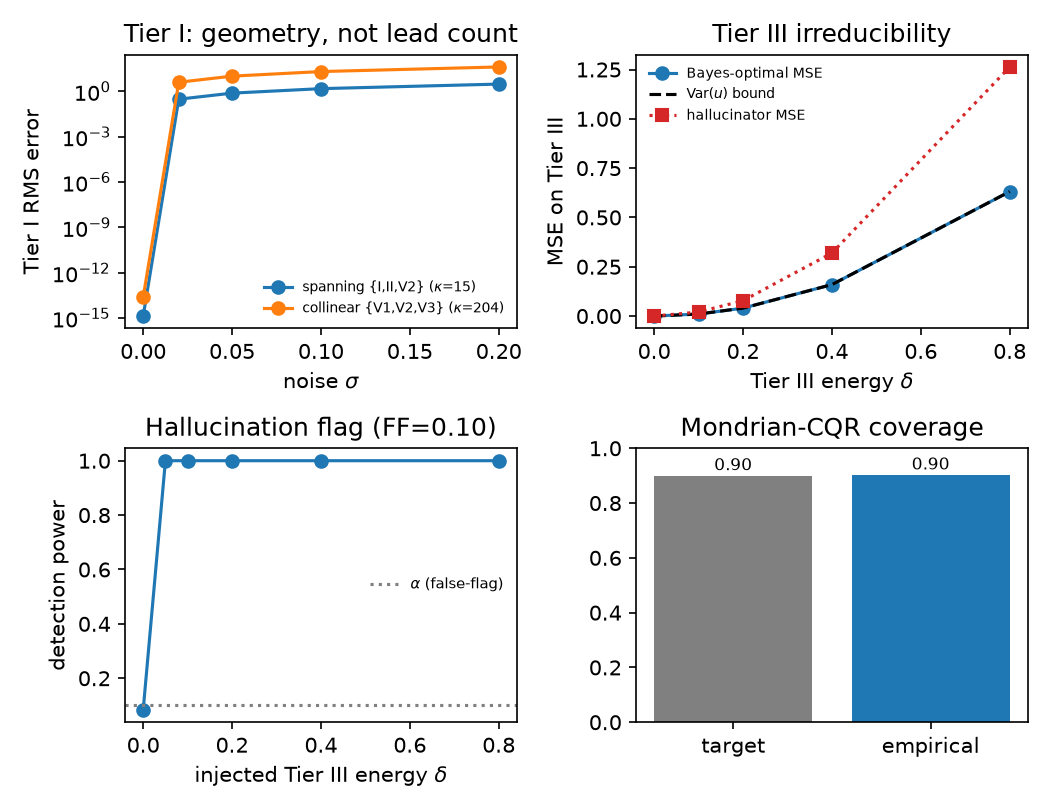
\includegraphics[width=\linewidth]{../results/synthetic_validation.png}
  \caption{Synthetic validation. Tier~I noise gain ($\kappa$); Tier~III
  irreducibility (Bayes $=\mathrm{Var}(\bm u)$; hallucinator $2\times$); flag power
  vs.\ false-flag rate; group-conditional coverage.}
  \label{fig:synth}
\end{figure}

\subsection{Geometry, not lead count}
On the PTB-XL QRS dipolar subspace, the closed-form gain $\kappa_s(S)$ ranks
configurations by \emph{conditioning}, not lead count: a single Lead~I observes only
one of three dipole directions (rank 1); a spread triplet $\{$I,\,II,\,V2$\}$ gives
$\kappa{=}\kapSpan$; three adjacent precordials $\{$V1,\,V2,\,V3$\}$ give
$\kappa{=}\kapColl$; but three \emph{coplanar} limb leads $\{$I,\,II,\,III$\}$ give
$\kappa{=}\kapCopl$ and the six limb leads $\kappa{=}\kapLimb$---so six frontal-plane
leads recover the (transverse) dipole far worse than three well-chosen ones.

\subsection{RMSE hides fabrication; the certificate reveals it}
Table~\ref{tab:hall} reconstructs the unobserved leads from $\{$I,\,II,\,V2$\}$ with
three methods. Their per-lead RMSE is nearly identical, yet the certificate separates
them. The dipolar baseline places \emph{zero} energy in the certified-unrecoverable
subspace ($h{=}0$): it never fabricates, but recovers only Tier~I. The learned linear
(OLS) reconstructor places moderate energy there that is \emph{positively correlated}
with the true non-dipolar content (it genuinely recovers Tier~II). The generative
reconstructor places the \emph{most} energy there, but that energy is
\emph{uncorrelated with truth} (correlation $\approx\genCorr$)---confident
fabrication that RMSE cannot detect and the certificate flags. The pattern is
identical across the Lead-I and limb-6 configurations (see \texttt{results/}).

\begin{table}[t]
\centering
\caption{Reconstruction from $\{$I,\,II,\,V2$\}$ on PTB-XL (fold 10). RMSE is matched;
the certificate's hallucination energy $h$ (mV) and non-dipolar correlation
$\rho$ with truth are not. Generative energy is uncorrelated with truth.}
\label{tab:hall}
\small
\begin{tabular}{llccc}
\toprule
seg & method & RMSE\,(mV) & $h$\,(mV) & $\rho$ \\
\midrule
\multirow{3}{*}{QRS}
 & dipolar     & 0.196 & 0.000 & $+0.00$ \\
 & OLS         & 0.196 & 0.030 & $+0.13$ \\
 & generative  & 0.228 & 0.097 & $+0.00$ \\
\midrule
\multirow{3}{*}{ST}
 & dipolar     & 0.125 & 0.000 & $+0.00$ \\
 & OLS         & 0.112 & 0.016 & $+0.28$ \\
 & generative  & 0.149 & 0.063 & $-0.00$ \\
\midrule
\multirow{3}{*}{T}
 & dipolar     & 0.140 & 0.000 & $+0.00$ \\
 & OLS         & 0.105 & 0.028 & $+0.44$ \\
 & generative  & 0.163 & 0.067 & $-0.00$ \\
\bottomrule
\end{tabular}
\end{table}

\begin{figure}[t]
  \centering
  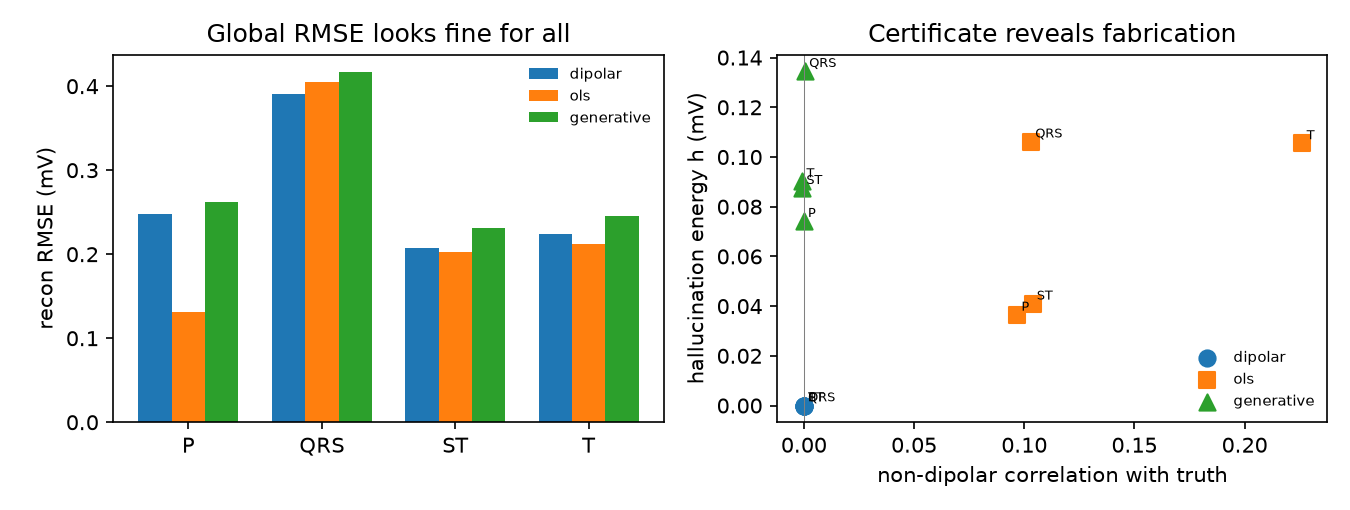
\includegraphics[width=\linewidth]{../results/ptbxl_hallucination.png}
  \caption{Left: global RMSE is similar for all reconstructors (limb-6$\to$precordial).
  Right: in the hallucination-energy vs.\ non-dipolar-correlation plane the generative
  model sits at high $h$, near-zero correlation---fabrication the certificate isolates.}
  \label{fig:ptbxl}
\end{figure}

\subsection{Safety case: precordial ST from limb leads}
The certificate warns \emph{before} reconstruction that limb-6$\to$precordial is
unsafe for an ST decision: $\kappa{=}\kapLimb$ and the ST segment is only $\dipST$
dipolar, so precordial ST is largely Tier~III. The danger is real and
\emph{bidirectional}. Over $799$ fold-10 records, measuring ST deviation (J$+$60\,ms
vs.\ the PR baseline, $0.1$\,mV threshold) on true vs.\ reconstructed V1--V6, the
generative reconstructor \emph{fabricates} $263$ phantom STEMIs (true signal negative),
whereas the conservative OLS reconstructor \emph{masks} $360$ real ones---opposite,
both-dangerous failures, at an identical $\sim\!0.075$\,mV mean ST error that RMSE
cannot separate. The per-reconstruction flag catches \emph{fabrication} (it detects
added, not missing, energy), abstaining on the highest-$h$ generative ST segments at a
controlled rate; masking is a property of the configuration, which the certificate's
$\kappa$ flags upfront. The lesson is the certificate's, not a single reconstructor's:
this configuration should not drive a precordial ST call. Counts in
\texttt{results/ptbxl\_stemi.json}.

\subsection{Guarantees under device shift}
Calibrating on the Schiller CS device family and testing on the AT family (a genuine
within-PTB-XL device shift), the ST/V4 interval keeps nominal $0.90$ coverage
in-distribution but drops to $0.82$ on the shifted device under plain conformal.
Weighted conformal \cite{tibshirani2019weighted} restores coverage (conservatively, to
$1.00$) and a $300$-record slice recalibration returns it to $0.93$
(\texttt{results/cross\_device.json}). Tier~I exactness and the Tier~III flag's
soundness are unaffected, as promised: only the Tier~II \emph{level} is shift-sensitive,
and it is both measurable and repairable.



\section{Conclusion}
Reduced-lead ECG reconstruction is not just ill-posed but ill-posed with a
\emph{known physical structure}. Exploiting the cardiac dipole turns ``trust the
reconstruction'' into a per-feature certificate: exact recovery where the dipole is
spanned, a calibrated interval where the population constrains the residual, and a
guaranteed flag where nothing does. The certificate separates reconstructors that
RMSE cannot, and catches fabricated ST elevations that a diagnosis would otherwise
inherit.

\bibliographystyle{IEEEbib}
\bibliography{refs}

\end{document}
